\section{V3}
\vspace{-0.5cm} 
\begin{multicols}{2}
    \begin{minipage}{\linewidth}
        \subsection{Halbleiter Speicher} 
        \textbf{Zentraler Speicher}
        \begin{itemize}
            \item direkt am Bussystem angeschlossen
        \end{itemize}
        \textbf{Peripherer Speicher}
        \begin{itemize}
            \item über I/O-Schnittstelle angeschlossen
        \end{itemize}
    \end{minipage}
    
    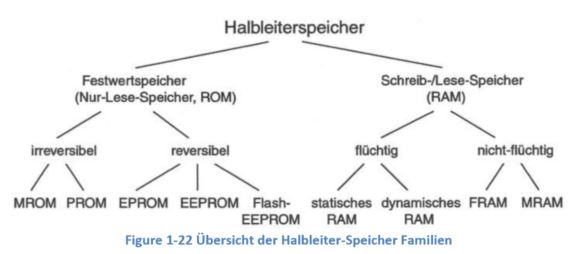
\includegraphics[width=1.1\linewidth]{images/halbleiterfam}
\end{multicols}

\vspace{-1cm} 
\begin{multicols}{2}
    \subsubsection{ROM-Festwertspeicher}
    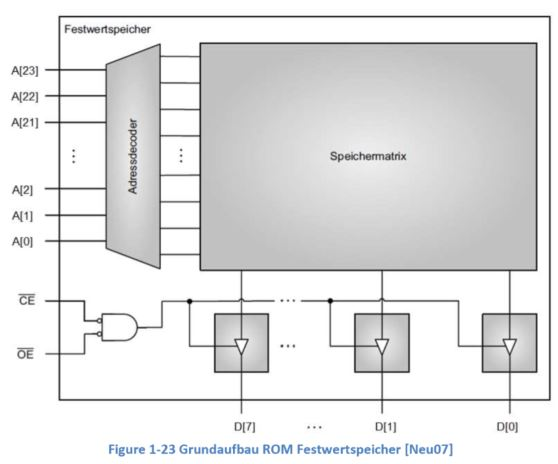
\includegraphics[width=8cm]{images/ROM}
    
    \subsubsection{RAM-Speicher-/Lese-Speicher}
    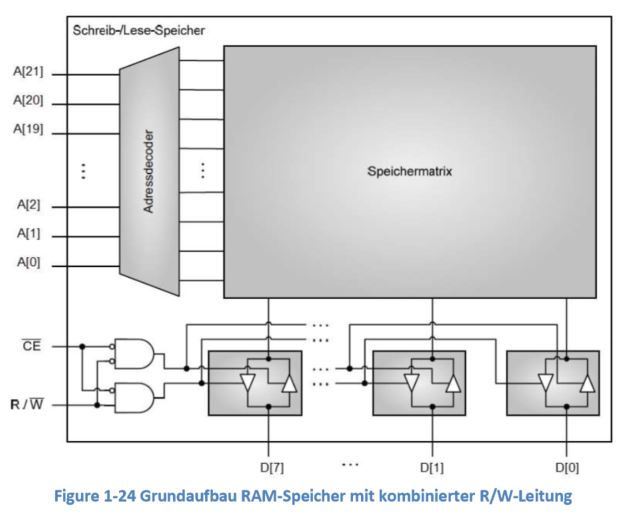
\includegraphics[width=8cm]{images/RAM}
\end{multicols}
    
\vspace{-1cm} 
\subsection{Speicherorganisation}
    
\begin{multicols}{2}
    \subsubsection{Little/Big Endian}
    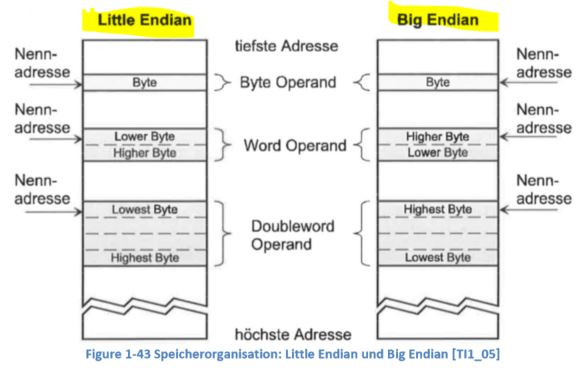
\includegraphics[width=8cm]{images/LittleBigEndian}
    
    \subsubsection{I/O - Schnittstelle}
    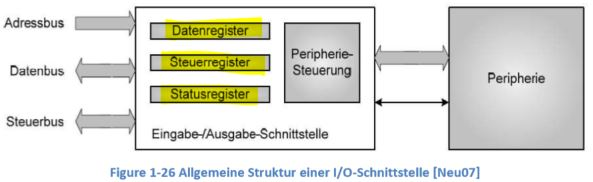
\includegraphics[width=8cm]{images/IOSchnittstelle}
\end{multicols}

\includegraphics[width=12cm]{images/Speicherraumadressierung}
\clearpage
%============================================

\section{Cortex}
\subsection{Cortex M Varianten}
\begin{multicols}{2}
    \textbf{Cortex M0 und M0+}
    \begin{itemize}
        \item kleinster Vertreter der CortexFam
        \item Ersatz von 8Bit- uC
    \end{itemize}                     
    \textbf{Cortex M1}
    \begin{itemize}
        \item als Softcore Implementiert
        \item Vergleichbar mit Cortex-M0
    \end{itemize}
\end{multicols}

\begin{multicols}{2}
   \textbf{Cortex M3}     
     \begin{itemize}
         \item erster Vertreter der CortexFam
         \item 32 Bit Architektur
         \item ersetzt 8 \& 16 Bit uC
         \item Thumb ISA (Instruction Set Architecure)\newline
         Mix aus 16 und 32Bit langen anweisungen
     \end{itemize}   
               
     \textbf{Cortex M4} 
     \begin{itemize}
        \item vergleichbar mit M3 jedoch mit:
        \subitem - Digital Signal Processing (DSP)
        \subitem - Floating Point Unit (FPU)
        \newline
      \end{itemize}  
\end{multicols}
\begin{multicols}{2}
    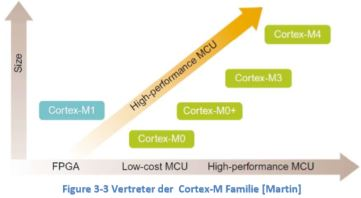
\includegraphics[width=\linewidth]{images/cortexmfam}
    
    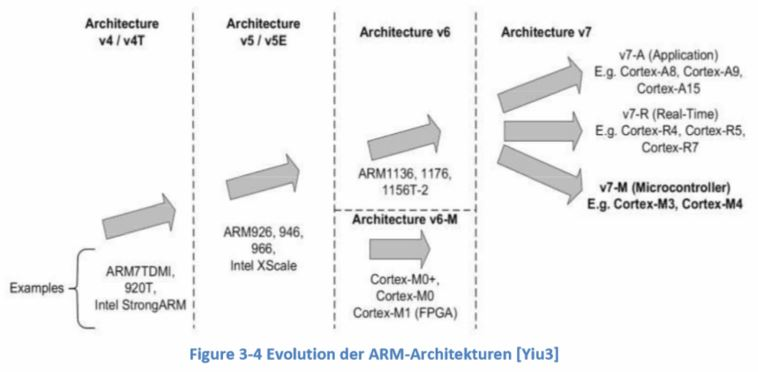
\includegraphics[width=\linewidth]{images/cortexmcomp}
\end{multicols}

\begin{multicols}{3}
\textbf{Cortex-A}
    \begin{itemize}
        \item HighEnd Anwendungen und Betriebssysteme
        \item hohe Rechenleistung
        \item Chache Memory
    \end{itemize}
    
    \textbf{Cortex-R}
    \begin{itemize}
        \item Echtzeitfähigkeit
        \item hohe Zuverlässigkeit
        \item System on Chip (SOC) 
    \end{itemize}  
    
    \textbf{Cortex-M}
    \begin{itemize}
        \item Speziell für \mu C-Markt
        \item Low Cost, Low Energy
        \item System on Chip (SOC) 
    \end{itemize}             
\end{multicols}

\subsubsection{Vorteile der Cortex-M-Prozessoren}
\begin{multicols}{2}
    \begin{itemize}
        \item Low Power
            \subitem < 200\mu A / MHz
        \item Performance
            \subitem >1.25 DMIPS / MHz
        \item Energy Efficiency
            \subitem low Power, high performance
        \item Code Density
            \subitem Thumb 2 Befehlssatz
        \item Interrupts
            \subitem 240 Interrupts
        \item Easy of Use, C Friedly
        \item Scalability
        \item Debug Features
        \item Software portability and Reusebility
        \item OS Support
        \item Choices (Derivers, Tools, OS,..)    
    \end{itemize}
\end{multicols}





















